Remembering that in chapter~\ref{ch:structure} it emerged some kind of structure behind data, where each tissue seemed to be sampled by a different power law, a topic modelling approach it is here proposed.

The idea is that behind data there are hidden variables that describe the relation between the genes and the samples. Let's call these variables topics.
Firstly it is necessary to build a bipartite network of genes and samples, than nodes are linked considering the gene expression value in the dataset.
\begin{figure}[htb!]
    \centering
    \includegraphics[width=0.7\linewidth]{pictures/topic/bipartite.pdf}
    \caption{An example of a bipartite network. Samples are on the left, genes are on the right. Each link is weighted by gene expression value. On the left side all nodes of the same colour are clusters of samples. On the right side all nodes with same colour are set of genes, also known as topics.\\ 
    Blue lines represent the cluster structure, each blue square is a set of nodes, lines delineate the hierarchical structure.\\
    It is clear in the middle the network separation in genes and samples.}
    \label{fig:topic/bipartite}
\end{figure}

The output of this kind of model are set of genes, the topics, with a probability distribution $P(gene | topic)$ and probability distributions of these topics inside each sample $P(topic | sample)$, both gives the relation between a \textit{sample} and a \textit{gene}.

\draft{gerarchico scrivi due righe!!}
\begin{figure}[htb!]
  \centering
  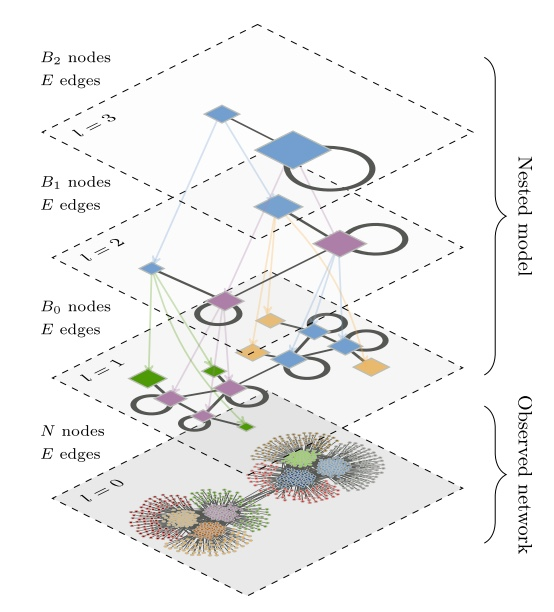
\includegraphics[width=0.6\linewidth]{pictures/topic/peixioto_hierarchic.jpg}
  \caption{Hierarchical structure}
  \label{fig:topic_peixioto_hierarchic}
\end{figure}

\draft{monte carlo scrivi due righe}
\begin{figure}[htb!]
  \centering
  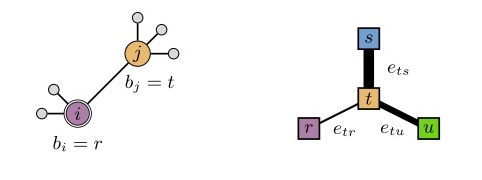
\includegraphics[width=0.9\linewidth]{pictures/topic/peixioto_move.jpg}
  \caption{Left: Local neighbourhood of node $i$ belonging to block $r$, and a randomly chosen neighbour $j$ \
  belonging to block $t$. \
  Right: Block multigraph, indicating the number of edges between blocks, represented as the edge thickness. \
  In this example, the attempted move $bi \to s$ is made with a larger probability than either $bi \to u$\
   or $bi \to r$ (no movement), since $e_{ts}>e_{tu}$ and $e_{ts}>e_{tr}$.}
  \label{fig:topic_pixioto_move}
\end{figure}

In this work it is used an innovative and recent approach to topic modelling, the algorithm was presented by~\cite{gerlach2018network} and extends the so called stochastic block models~\cite{Holland1983}. 
Topic modelling is being developed and studied to approach linguistics problems, so this algorithm was developed considering words and books as input, links represents the abundance of a word in a book. In chapter~\ref{ch:structure} was evident that there are many similarities between data considered in this work and linguistics' dataset. Referring to data used in this project documents will be \textbf{samples}, words will be \textbf{genes}.
It is expected that topics represent some properties of samples due to the gene expression distribution in samples.

The ultimate goal would be to be able to separate healthy and diseased samples, than separate and find well known tumour types, than extend the actual knowledge and retrieve the tumour sub-types.

See~\ref{app:hsbm} for detailed analysis of the math behind the algorithm and \url{https://cloud.docker.com/repository/docker/fvalle01/hsbm} for the extension of~\cite{gerlach2018network} to non linguistics component systems datasets.